% define document type (i.e., template. Here: A4 APA manuscript with 12pt font)
\documentclass[man, 12pt, a4paper]{apa7}

% add packages
\usepackage[american]{babel}
\usepackage[utf8]{inputenc}
\usepackage{csquotes}
\usepackage{hyperref}
\usepackage[style=apa, sortcites=true, sorting=nyt, backend=biber, natbib=true, uniquename=false, uniquelist=false, useprefix=true]{biblatex}
\usepackage{authblk}
\usepackage{graphicx}
\usepackage{setspace,caption}
\usepackage{subcaption}
\usepackage{enumitem}
\usepackage{lipsum}
\usepackage{soul}
\usepackage{xcolor}
\usepackage{fourier}
\usepackage{stackengine}
\usepackage{scalerel}
\usepackage{fontawesome}
\usepackage[normalem]{ulem}
\usepackage{longtable}
\usepackage{amsmath}
\usepackage{afterpage}
\usepackage{float}
\usepackage{titling}
\usepackage{censor}

% formatting links in the PDF file
\hypersetup{
pdfpagemode={UseOutlines},
bookmarksopen=true,
bookmarksopenlevel=0,
hypertexnames=false,
colorlinks   = true, %Colours links instead of ugly boxes
urlcolor     = blue, %Colour for external hyperlinks
linkcolor    = blue, %Colour of internal links
citecolor   = cyan, %Colour of citations
pdfstartview={FitV},
unicode,
breaklinks=true,
}

% language settings
\DeclareLanguageMapping{american}{american-apa}

% add reference library file
\addbibresource{references.bib}

% Title and header
\title{Supplemental Information D: Context of the Migration Experience Framework}
\shorttitle{SI D: Acculturation Context}
\author{Jannis Kreienkamp, Laura F. Bringmann, Raili F. Engler, Peter de Jonge, Kai Epstude}
%\author{[authors masked for peer review]}

% set indentation size
\setlength\parindent{1.27cm}

% adapt table and figure labels
\setcounter{equation}{0}
\setcounter{figure}{0}
\setcounter{table}{0}
\setcounter{page}{1}
\makeatletter
\renewcommand{\theequation}{S\arabic{equation}}
\renewcommand{\thefigure}{S\arabic{figure}}
\renewcommand{\thetable}{S\arabic{table}}

% Start of the main document:
\begin{document}

% add title information (incl. title page and abstract)
\begin{titlepage}
	{\noindent\Large Supplementary Information for \par}
	\vspace{0.5cm}
	{\noindent\Large The Migration Experience: A Conceptual Framework and Systematic Scoping Review of Psychological Acculturation\par}
	\vspace{1.5cm}
	{\noindent\LARGE\bfseries \thetitle \par}
	\vspace{2cm}
	{\noindent\Large\itshape \theauthor \par}
	\vfill
	\noindent Corresponding Author: Jannis Kreienkamp\par
	\noindent E-mail: j.kreienkamp@rug.nl\par
	%\noindent Corresponding Author: [masked for peer review]\par
	%\noindent E-mail: [masked for peer review]\par
	\vfill

    % Bottom of the page
	{\noindent Last updated: \today\par}
\end{titlepage}

% add title again on page 1 (after title page)
\begin{center}
   \textbf{\thetitle} 
\end{center}

This supplementary information elaborates on the background literature of the contextual aspects of our conceptual framework presented in the main text. We would like to address each of the four contextual factors in more detail: (1) Cultures, (2) individuals, and (3) situations.

%\begin{figure}[h]
%\centering
%\caption{Conceptual Model with Context.}
%\includegraphics[width=\textwidth]{Figures/ConceptualFrameworkStatic.pdf}
%\label{fig:SupModelContext}
%\end{figure}

\begin{sidewaysfigure}
    \centering
    \caption{Conceptual model with context and experience process. The process diagram shows the main elements with examples for each conceptual building block.}
    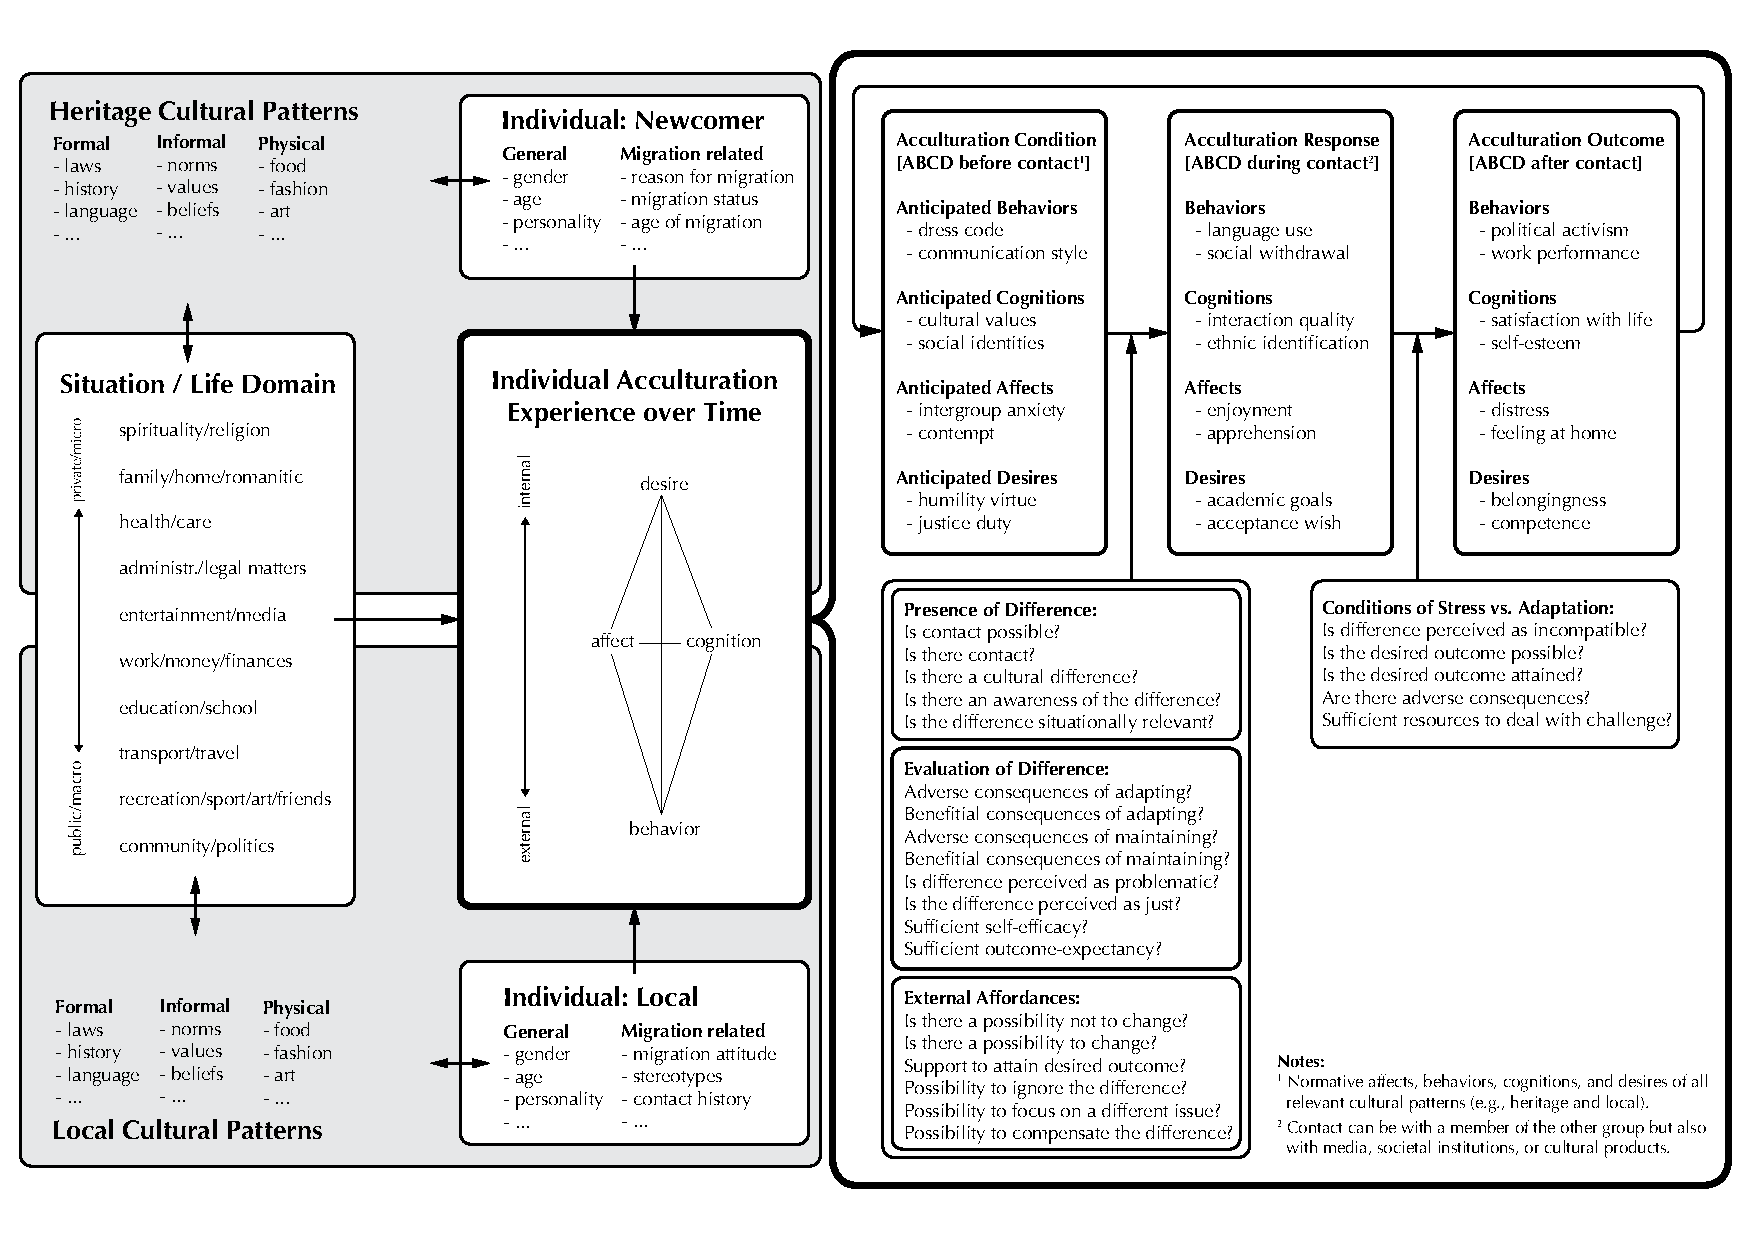
\includegraphics[width=\textwidth]{Figures/ConceptualFrameworkExpandedOptima_Revision.pdf}
    \label{fig:SupModelContext}
\end{sidewaysfigure}

\section{Culture} 
% Culture as social facts and Cultural adaptation as tension between different social facts.
The most prominent contextual factor of psychological acculturation is probably the concept of culture. In the main text, we already discuss our conceptual approach to cultural patterns. As part of the analyses presented in this paper, we will offer such a review reflection by extracting the countries of origin and settlement for which acculturation measures were validated and investigated in empirical papers. While this does not reflect the full complexity of cultural patterns, it is a commonly used proxy available for most empirical works. This allows us to examine how much the cultural contexts are reflected within structural differences of measures and definitions (that is if we can consolidate a meaningful number of studies per cultural context).

\section{Situation} 
%% Situations as domains of psycho-social functioning: 
% Many theories have come up with life domains that form different cultural interaction situations.
Beyond the cultural patterns, the interactions of cultural adaptation are further dependent on the situational context. As part of the main manuscript we already introduce a conceptual discussion of the contact context. What structurally unites the different conceptualizations of life domains is the dimension of closeness to the individual. That is, most areas of life found in the literature can be arranged from the most immediate (i.e., micro or private, such as family) to the broadest levels (i.e., macro or public, including government or media). So, based on sociological theories of social institutions \citep{Durkheim1982}, literature on life domains in acculturation \citep{Arends-Toth2006, Arends-Toth2007, Zane2004}, a categorization of psychological influences by the British Psychological Society \citep{Michie2005a}, and Bronfenbrenner's Ecological systems theory \citep{Bronfenbrenner1992}, we conceptualized a range of life domains relevant to the migration process (also see Figure \ref{fig:SupModelContext}). As part of this study, we extracted information on which of these domains was assessed in the methodological and empirical literature. We then assess whether different foci on life domains also show differences in their understanding and measurement of affective, behavioral, cognitive, and motivational acculturation.

\section{Individual} 
% Individual differences in general (e.g., age, gender) but also migration related differences (e.g., reason for migration, language proficiency)
A final contextual factor we consider during the cultural adaptation process are the involved individuals themselves. Although it can, at times, be difficult to disentangle cultural from individual influences, there is a range of personal features that likely influence the cultural adaptation process. These personal differences might relate to relatively stable individual differences, such as gender or personality, but also migration-related differences, such as the reason for migration (e.g., voluntary vs. forced migration), cultural distance, or migration status. Within the migration-related factors, we would also include aspects that might change over the course of the adaptation process but give migrants different starting positions, such as language skills and education level.
Similar to the influences of cultural patterns, the individual differences of the interaction partners (if there are multiple people) will likely impact the psychological acculturation process. And similar to cultural patterns, individual differences likely play a role in multiple aspects of the cultural adaptation process (also see Figure \ref{fig:SupModelContext}). As part of this study, we will mainly analyze the migration-relevant differences. Considering individual differences on a larger, cross-study level we will mainly extract data on the type of samples collected within the validation and the empirical papers (e.g., forced vs. voluntary, youth, or clinical samples). If we find reasonable numbers of studies with specific types of samples, we will assess whether these individual differences are related to structural differences in measures or definitions used by the authors.

\section{Measurement}
As part of our efforts to capture the migration context, we were interested in cultural, individual, situational, as well as process-related contexts. Assessing these contexts in a manner that is relevant across a wide range of studies is challenging and likely superficial at best. Yet gaining a more general understanding of the contexts frequently considered in the literature could prove useful in evaluating and comparing conceptions of cultural adaptation. We, thus, extracted a range of general context variables from the empirical literature.

\subsection{Cultural Context}
To capture the cultural contexts researched, we coded both the heritage country of the migrants as well as the country of the receiving host society. Coding the two societal contexts allows us to extract information on the specificity of the studies (e.g., Mexican migrants in the United States, vs any migrant in Scandinavia). Migrant and host country coding could also reveal patterns of interest within the literature (e.g., common migrant groups, common host societies, or common combinations investigated). And finally, if common clusters emerge, we could compare the types of experience elements assessed within each cluster (e.g., focus on behavioral adaptation in one and cognitive focus in another cluster). Note that we do not seek to equate nationalities, nations, or regions with culture. Instead, country of origin and country of settlement are the only consistently reported markers of cultural contexts and we thus only treat them as a surface-level proxy to assess the common patterns within the literature.

\subsection{Sample}
To capture the individual background on a cross-paper level, we extract the types of samples recruited by the authors. Some studies might focus on young or elderly samples, men or women only, clinical samples, or authors might simply recruit any migrant from a certain country or region. Clusters and differences in the experience foci within these clusters might offer insights into the understanding of cultural adaptation for different individual contexts.

\subsection{Life Domains}
To capture the situational contact focus of the authors, we coded which life domains the scales referred to. There is a range of ways in which we could identify the domains the authors wished to cover. Often times authors will explicitly mention which life domains their measure aims to capture. Others will mention clear domain focus as part of sub-scale or factor labels. If there is no explicit mention by the authors, questions are likely worded to refer to a specific life domain (e.g., behaviors at school, or values in the family context). If there is no clear reference to a life domain or the questions are about life in general, we code this as meaningful information as well. We can then process the situational foci as a list of domains, which offers information on the diversity of domains (e.g., number, or similarity of domains) but also the focus in the literature in general (e.g., frequency of domain across all articles). If clusters of similar focus domains emerge, we could, additionally, assess differences in the assessment of cultural adaptation for these clusters.

\section{Results}
% import methods and results from R Markdown (in file: "Supplemental-Material-E-Results.tex")
\input{Supplemental-Material-D-Results.tex}

\section{Discussion}
Within this supplemental material, we assessed contextual differences that were captured within the methodological and empirical literature on psychological acculturation. We focused particularly on the regional and national groups recruited to assess cultural foci, the samples recruited to capture individual differences that were sampled, as well as the life domains considered in the acculturation measures to investigate situational focus points. Across all three contextual factors, we find an enormous heterogeneity. Few studies seem to cluster around the same contexts. And while we see that there is less diversity within the methodological literature, neither the methodological nor empirical literature allowed us to identify meaningful clusters to compare experience assessments across contexts.

\printbibliography

\end{document}